\documentclass[12pt]{article}
\usepackage{mathpazo}
\usepackage{graphicx}
\usepackage[explicit]{titlesec}
\usepackage{hyperref}
\usepackage[export]{adjustbox}
\usepackage{placeins}
\usepackage{subcaption}
\usepackage{import}
\usepackage[dvipsnames]{xcolor}
\usepackage{listings}
\usepackage{setspace}
\usepackage{rotating}

\begin{document}
\onehalfspacing
%title page
\begin{center}
	{\huge {\textbf{Politecnico di Milano}}}
	 	\vspace{7mm}\\
	 	
 	 	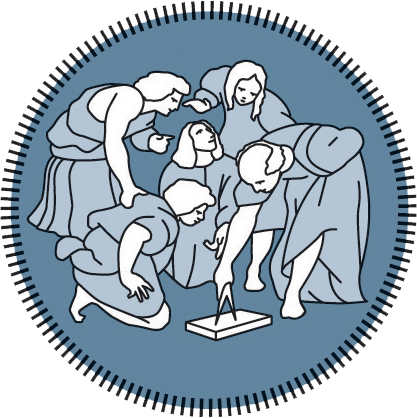
\includegraphics[scale=1.5]{Images/PolimiLogo.png}
	\end{center}

\begin{center}
	     \vspace{5mm}
		{\Large A.A 2019/2020} 
		\vspace{1cm}\\
		{\Large {\textbf{Design Document}}}   
		
\includegraphics[scale=1]{Images/LOGO.jpg}
    \end{center}
          
\begin{flushright}
         
	 	 
	 	{\huge {\Large \textbf{Authors:}}}
	 	 
	 	{Armenante Valerio}
	 	
	 	{Capaldo Marco}
	 	
	 	{Di Salvo Dario}
	\end{flushright}


%begin of contents

\newpage
\hrule
\hypersetup{hidelinks}\tableofcontents

\vspace{0.5mm}
\vspace{0.24mm}

\newpage

\section{Introduction}
\hrule
\vspace{1cm}
\subsection{Purpose}
\vspace{5mm}
In the presented document is the Software Design Document where there is a general view of the SafeStreets platform presented by the
RASD, with all the functions that the system has to realize and to give implementative and technical details. Specifically, this document wants to concentrate on the analysis with high level descriptions of the main aspects, describe
the architectural styles and pattern, and generally establish the design standards for the development phase of components, run-time processes, deployment. All the informations that are going to be written in this document are also intended to behave as a guide to
follow during the software developing process.
The document will pursue the analysis following a rigorous scheme, to make a clear and complete description about these characteristics of the software.
In particular, this document is intended for stakeholders, software engineers, and programmers and must be used as reference throughout the whole development of the system. The document is going to present an overview of the high level architecture, together with an explanation of the main components and the communication system between them through their interfaces; the description of the runtime behavior together with an overview of the deployment mechanism; the definition of the design patterns of the most crucial parts of both the mobile application and web application; the definition of the implementation, integration and testing plans.

\subsection{Scope}
\vspace{5mm}
As presented in the RASD Document, the SafeStreets software allow users to notify traffic violations to authorities. More specifically, the notification process consists in the acquisition of pictures, date, time, location and type of reported violation inserted by user. The aim of SafeStreets basic service is to retrieve and store information from inputted data, completing it with suitable metadata.  In particular, when user sends pictures related to a traffic violations, SafeStreets is able to recognize license plate by means of an external algorithm. After that, SafeStreets dispatches the notification to the authority member, which is in an available status and is chosen according to the minimum distance between the notified traffic violation and authority member’s position. In the end, the assigned authority member will opportunely manage the received request. In addiction, users and authorities member, through a Mobile Application interface presenting different level of visibility to different roles, will be able to mine information that has been received, for example by highlighting the areas with the highest frequency of violations. This is going to be realized designing some algorithms able to generate statistics on the previously stored data. A user who approaches the mobile application for the first time has to complete a registration process, as well as an authority which approaches the dedicated website for the first time. In particular, an authority inserts all their authority member in SafeStreets database through a website’s form specifying their e-mail and unique code. In this way, each authority member have to do only an activation process, inserting their personal data and the assigned unique code.
Thanks to the first advance function, the software is able to improve more the security of cities through a cooperation with municipality. First of all SafeStreets retrieves information from municipality through an external service, then information are categorized (accidents, violations, etc.) and some statistics are generated. Then crossing information between resultant elaboration and already available SafeStreets data, the goal can be reached. More specifically, if traffic violations cardinality, related to an area, exceed a specified threshold, SafeStreets identifies the area as unsafe and suggests possible interventions to municipality. Obviously, the threshold is properly defined according to the characteristics of the city.
Then through the second advance function, SafeStreets can provide correct information, related to traffic violations, to municipality(in particular local police). In this way, municipality can easily and correctly emits traffic tickets to the offenders. In order to ensure the correctness of information, SafeStreets implements an algorithm that recognize if a manipulation is occurred on uploaded data by users. Moreover, Safestreets builds some statistics regarding traffic tickets data such as a ranking of the most offenders, most common violations and the effectiveness of SafeStreets initiative.
\vspace{1cm}

\newpage
\subsection{Definitions, Acronyms and Abbrevations}
\vspace{5mm}
\subsubsection{Acronyms}
\vspace{5mm}

\begin{flushleft}

\textbf{RASD} - Requirements Analysisand Specifications Document
\vspace{3mm}

\textbf{DB} - Database
\vspace{3mm}

\textbf{DBMS} - Database Management System
\vspace{3mm}

\textbf{API} - Application Programming Interface
\vspace{3mm}

\textbf{DD} - Design Document
\vspace{3mm}

\textbf{GUI} - Graphical User Interface
\vspace{3mm}

\textbf{MVC} - Model View Controller is a designed pattern used for GUIs
\vspace{3mm}

\textbf{JDBC} - Java DataBase Connectivity
\vspace{3mm}

\textbf{RMI} - Remote Method Invocation
\vspace{3mm}

\textbf{PC} - Personal Computer
\vspace{3mm}

\textbf{HTML} - Hyper Text Markup Language
\vspace{3mm}

\textbf{CSS} - Cascading Style Sheets
\vspace{3mm}

\textbf{AM} - Authority Member
\vspace{3mm}

\end{flushleft}

\subsubsection{Abbreviations}
\vspace{5mm}
\begin{flushleft}
\textbf{Gn} - n-Goal

\vspace{1.5mm}
\textbf{Rn} - n-functional Requirement
\end{flushleft}
\subsection{Revision History}
\vspace{5mm}
TBU
\subsection{Reference Documents}
\vspace{5mm}
This Design Document is directly linked to the Data4Help RASD v2.0 document.
\subsection{Document Structure}
\vspace{5mm}
\newpage
\section{Architectural Design}
\hrule
\vspace{1cm}
\subsection{Overview: High-level components and their interaction}
\vspace{5mm}
\begin{center}
\includegraphics[scale=0.40]{Images/ARCDIAGRAMOK.jpg}
\vspace{2mm}

Figure 2.1: Physical architecture diagram.
\end{center}
\vspace{3mm}
The high level architecture of the system is divided in three main layers or tiers (as shown in figure 2.1):
\begin{itemize}
\item \textbf{Client-side layer}: this is the closest part of the system to the customers: authority member, authority and user's interfaces. It is composed by the customer mobile application, and the authority web application.

\item \textbf{System core network layer}: identifies the central portion of the infrastructure, the "mind" of the system. It is composed by the Application Server, which is protected by Firewalls, and by the System Manager Web Application, which owns a direct interface to the Application Server and monitor all the functionality aspects of the system.

\item \textbf{Storage layer}: identifies the storage tier of the infrastructure, where there are all the backups of the data of our system. It is composed by the Database Server, SafeStreets Data Database and Administration Database.
\end{itemize}
The System core network layer is composed by the the Application Server, the “mind” of the system, that is protected in an efficient and secure way thanks to firewalls placed before the communication with the internet network , the Database Server and the System Manager Web Application.
The System Manager have to monitor the Application Server with the aim to manage
events into the system, for example Request of Data Access like statistic's data or other type of data saved in the system itself, or the Registration Request of new customer and so on.
Furthermore, the System Manager can access to the Storage layer through the Application Server and manage the data in the Database.
The Customer Mobile Application is the User client front-end portion of the system, that owns
an interface to the Mobile Data Network, through which the client can access to the Internet
network and can use the services offer by the system.
The Database Server receives and manages every incoming request, which regards one of the storage entities among SafeStreets Data Database and Administration Database (it holds
Data about subscribed Authorithy, Authority Member, User  and other relevant administration-oriented data). The system is completely oriented towards data integrity and persistence thanks to the Backup Database Server.

\subsection{Component view}
\vspace{5mm}
\begin{center}
\includegraphics[scale=0.24]{Images/UMLok.jpg}
\vspace{2mm}

Figure 2.2: SafeStreets Class Diagram.
\end{center}

\newpage
\subsubsection{High Level Component Design}
\vspace{5mm}
In the figure 2.3 there is presented an high level Component Diagram about interfaces provided by the Server Side of the application, Authority Web Services, System Manager Web Services and SafeStreets Mobile Services. The Authority Web Services and the System Manager Web Services interacts with the Web Application client side, while the SafeStreets Mobile Services interacts with the Mobile Application client side. An unique mobile application is provided to Customers while two different web application are intended for the System Manager and Authority.
\begin{center}
\includegraphics[scale=0.5]{Images/CDOK2.jpg}

\vspace{2mm}
Figure 2.3: SafeStreets High Level Component Diagram.
\end{center}

\newpage
\begin{flushleft}
\emph{Authority Web Services} - provides the interface to permit Authority to perform Data Access Request and manage Data.
\vspace{2mm}\\
\emph{System Manager Web Services} - provides the interfaces to System Manager to perform manintenance and updates tables, occurred Subscriptions and evaluating Data Access Requests.
\vspace{2mm}\\
\emph{SafeStreets Mobile Services} - provides the interfaces that permit Customers to exploit all the SafeStreets services.
\end{flushleft}

\subsubsection{SafeStreets Mobile Services projection }
\vspace{5mm}


SafeStreets Mobile Services subsystem is composed by more components and two different interfaces are exposed to the Mobile Client that are Retrieve Data Service and Customer Activity Service. The Customer Activity Service interface is given by the  Customer Control Activity component, that is able to router the activities among User, Authority and Authority Member and to manage the Login and Registration/Authentication Processes. For the User, the Customer Control Activity component will show all the component interfaces referring to the SafeStreets application. First of all for the User there is the Profile Manager component which its Profile Service interface is used to manage the User Profile. User is able to interface to the Notification Component and then notify the Authority Member about a violation, through the specific interface Violation Data Service. The User can also complete  info about a alleged violation during the Notification phase,like time, and position using a maps API thanks to the component Device Data Manager and its interface Data Service. The User can also gets info about statistics thanks to the Statistics Data Service interface of the component Statistics Data Manager. The Customer Control Activity component gives to the Authority Member the possibility to access more components than the User. AM can access to the interface Profile Service to manage his profile and also set his Availability Status thanks to the interface Availability Status Service and its component Availability Status Manager. AM can also manage in an efficient way the received notification through the interface Violation Service and gets info about Statistics through the interface Violation Service and respectively interfaces. Also AM can sent the verified violation and relative info thanks to the Ticket Manager component to the Authority. The Customer Control Activity component also exploit the interfaces relative to the Authority. Authority can access also the interface Profile Service, manage its list thanks to the AM List Service Interface. Moreover the Authority can administrate the tickets thanks to the Ticket Service.
In order to pursuit their goal every components need to communicate with the DBMS, in particular the Tickets Manager communicate with the FindOwnerPlate.

\begin{center}
\includegraphics[scale=0.59]{Images/componentMobile.jpg}

\vspace{2mm}
Figure 2.4: SafeStreets Mobile Services projection.
\end{center}


\subsubsection{Authority Web Services projection}
\vspace{5mm}
In the component diagram of the Authority Web Services subsystem are presented the principal components and interfaces. At the first sight there is the Authority Profile Manager that act as the main component and exposes the Authority Web Service interface to the Web Client in order to fullfill the purpose of the application exploiting the interfaces of the Data Request Manager, Ticket Manager and the AM List Manager.The Data Request Manager is intended to perform the Data Access Request, the Ticket Manager provides the feature for managing a ticket’s emission and the AM List Manager component to organize and modify the table lists about the authority’s employeees. Certainlty all the components of the subsystem needs to communicate with the DBMS.
\begin{center}
\includegraphics[scale=0.59]{Images/componentWebA.jpg}
\vspace{2mm}
Figure 2.5: Authority Web Services projection.
\end{center}
\vspace{3mm}
\subsubsection{System Manager Web Services projection}
\vspace{5mm}
This subsystem is similar in the architectural pattern point of view as the Authority Web Services subsystem. The System Manager Activity Profile exposes the three main interfaces that enable Authority to access the three corrispondent main components: System Data Manager, System Statistics Manager and System AM List Data Manager.
Thanks to these components the Authority can modify the AM' list, access and update the Statistics and manage also the activity made by the System Manager as authorize the login, signup and authentication. The System Manager can notify the municipality about the improvements thanks to the infos gets by the statistics.


\begin{center}
\includegraphics[scale=0.59]{Images/componentWebSOKK.jpg}

\vspace{2mm}
Figure 2.6: System Manager Web Services projection.
\end{center}


\newpage
\subsection{Deployment View}




\begin{center}
\includegraphics[scale=0.40]{Images/deploymentview.jpg}


\vspace{2mm}
Figure 2.7: Deployment view.
\end{center}
\vspace{3mm}
There is a description of the main three tiers in Figure 2.7:

\begin{itemize}
\item The first tier is the \emph{Client-side} one. In this tier there are the Mobile application and the Web Application. These two applications communicate directly to the Application Server using the RMI systems. The Mobile phone application is designed for the User, AM and Authority phones, while the Web Application is thought for Authority PC. The recommended implementation of the Mobile Application have to suits  Android, iOS operative systems. For the Web Application development is recommended the HTML5,JavaScript and CSS.
\item The second tier is the \emph{System core network} tier. In this tier there is the Application Server, consisting in Apache TomEE 5.0.0, running on a Linux OS which act as a Web Server, script engine Web Servlet and Web JSP modules. It receives RMIs from the Mobile Application and HTTP messages from the Web Application.
\item The third tier is the \emph{Storage} one, which consists of a DB server, Oracle Database 19c, linked to each storage entity involved into the system. This server communicate with the Application Server through JDBC protocol.
\end{itemize}
\vspace{5mm}

\subsection{Runtime View}
\vspace{5mm}

In the following sequence diagrams there is the description about the interactions between the components and the requests handled by them during the execution of the main features. Is better to specify that this is a high-level description, so functions and their names may be modified or named in another way  during the implementation process.

\subsubsection{User Send Notification}
\begin{center}
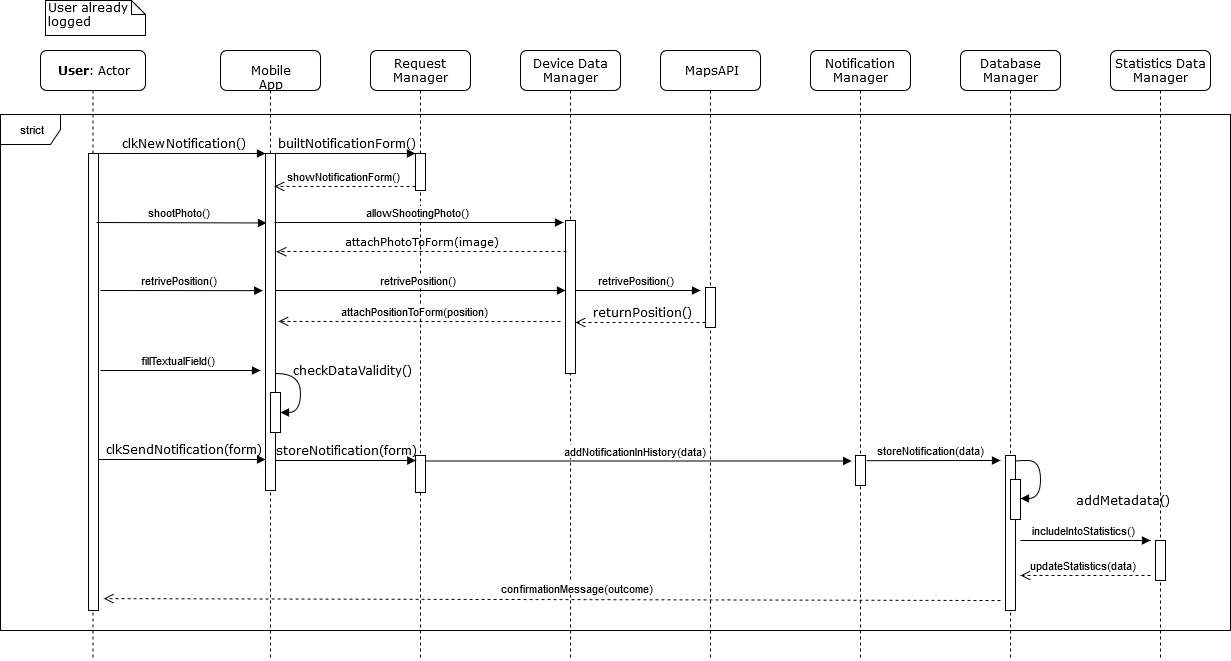
\includegraphics[scale=0.40]{SequenceDiagram/userSendNotification.jpg}


\vspace{2mm}
Figure 2.8: User send notification runtime view.
\end{center}
\newpage
\subsubsection{Authority Member receives Notification}
\begin{center}
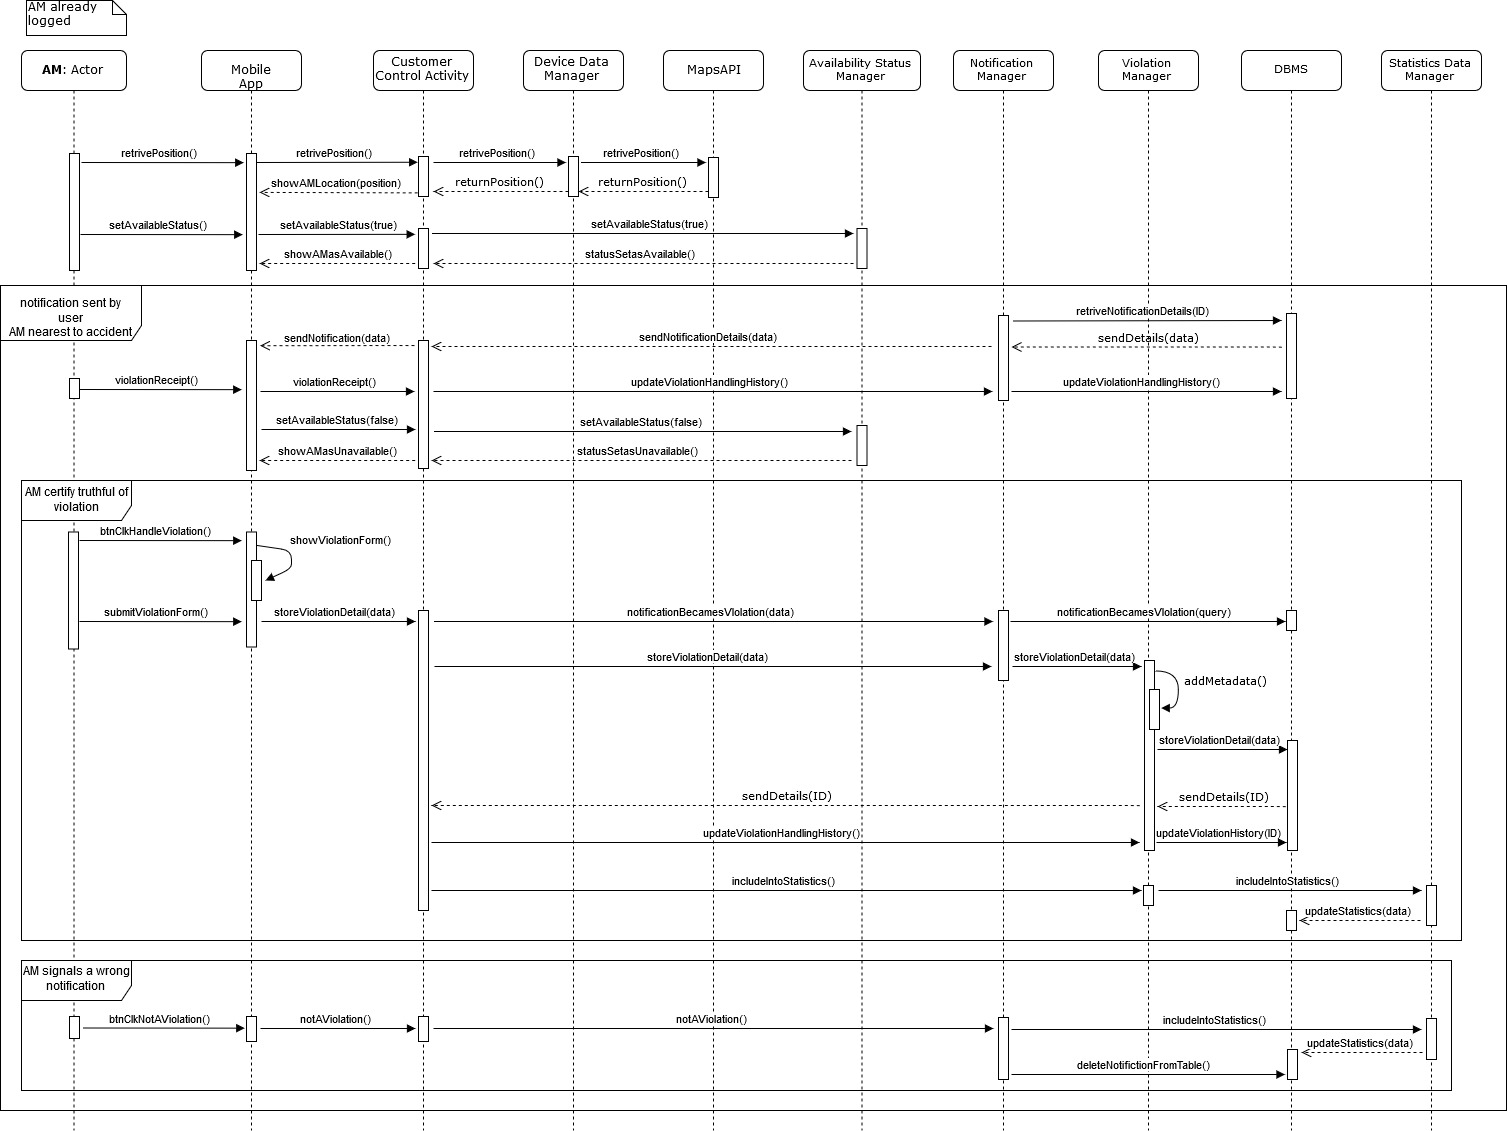
\includegraphics[scale=0.30]{SequenceDiagram/authorityMemberReceiveNotification.jpg}


\vspace{2mm}
Figure 2.9: AM receives Notification runtime view.
\end{center}
\newpage
\subsubsection{Authority Member past Notification}
\begin{center}
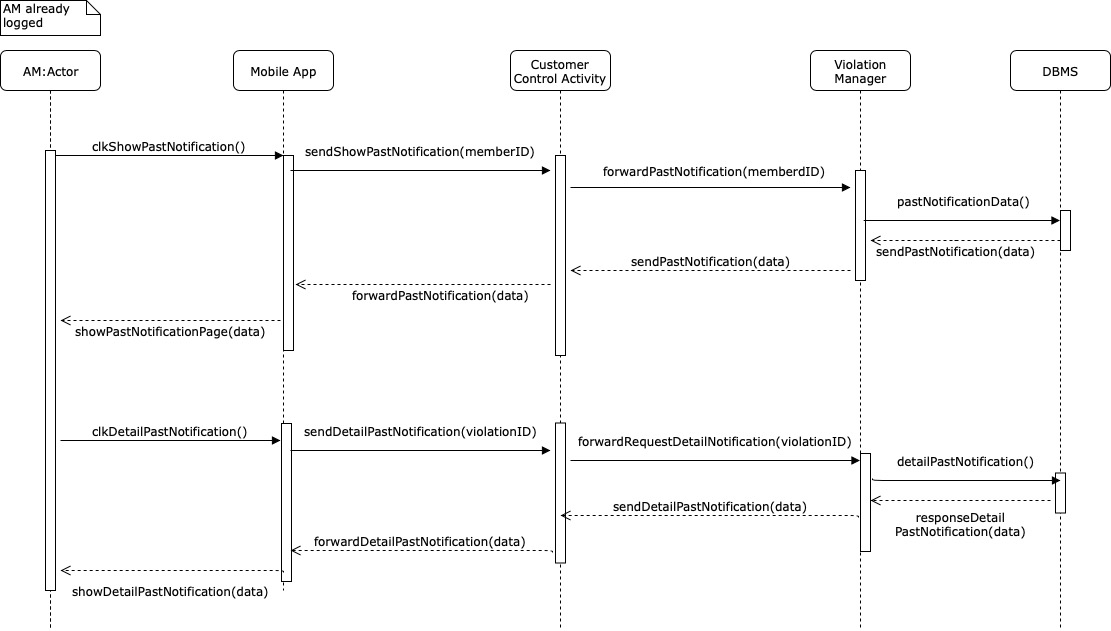
\includegraphics[scale=0.30]{SequenceDiagram/AMPastNotification.jpg}


\vspace{2mm}
Figure 2.10: AM past Notification runtime view.
\end{center}
\subsubsection{Authority Ticket generation process}
\begin{center}
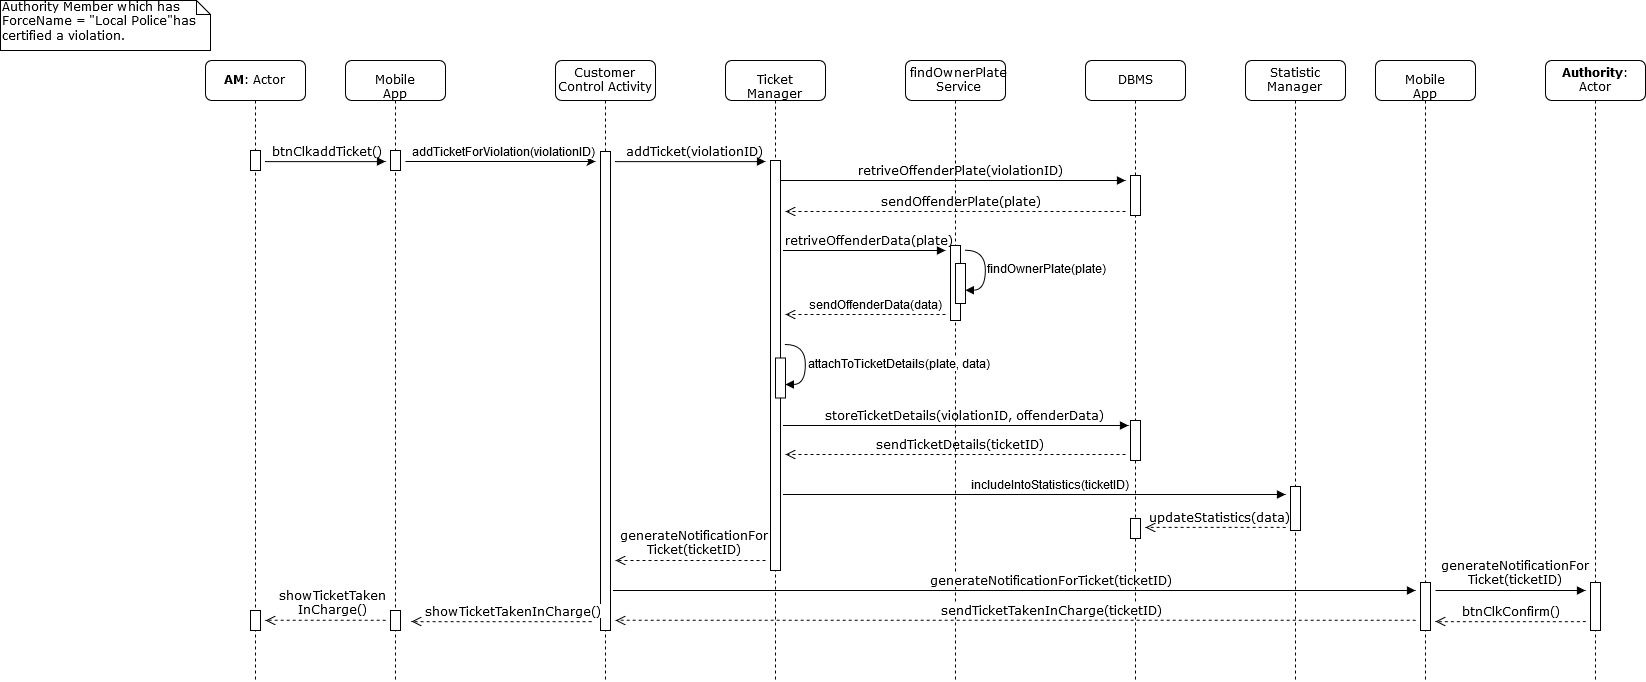
\includegraphics[scale=0.28]{SequenceDiagram/ticketGenerationProcess.jpg}


\vspace{2mm}
Figure 2.11: Authority Ticket generation process runtime view.
\end{center}
\subsubsection{User accesses Statistics}

\begin{center}
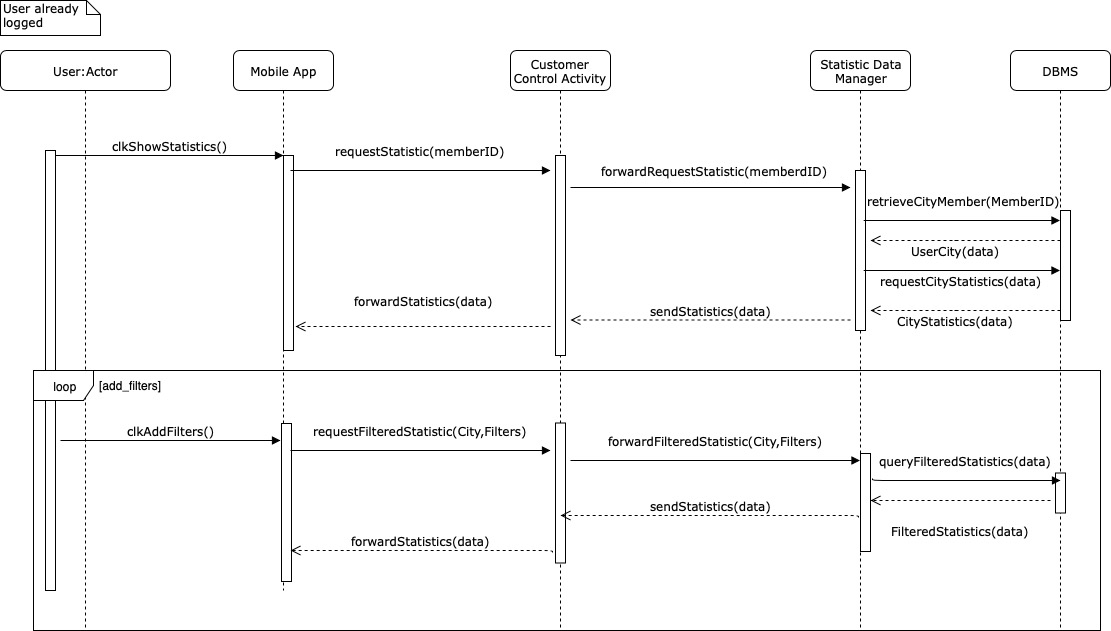
\includegraphics[scale=0.28]{SequenceDiagram/UserStatistics.jpg}


\vspace{2mm}
Figure 2.12: User accesses Statistics process runtime view.
\end{center}

\subsubsection{System sends Suggestions}
\vspace{2mm}
\begin{center}
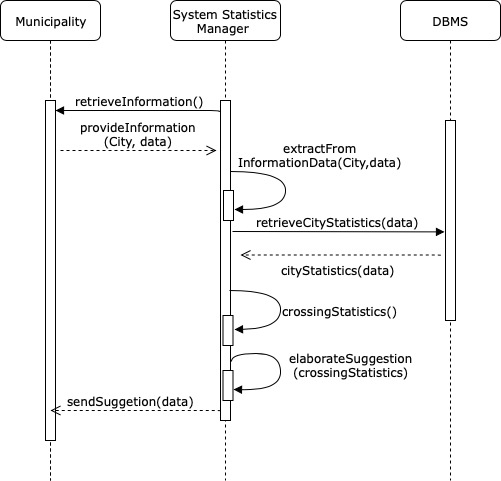
\includegraphics[scale=0.45]{SequenceDiagram/municipalitySuggestion.jpg}


\vspace{2mm}
Figure 2.13: System sends Suggestions runtime view.
\end{center}

\newpage
\subsection{Component Interfaces}

\begin{center}
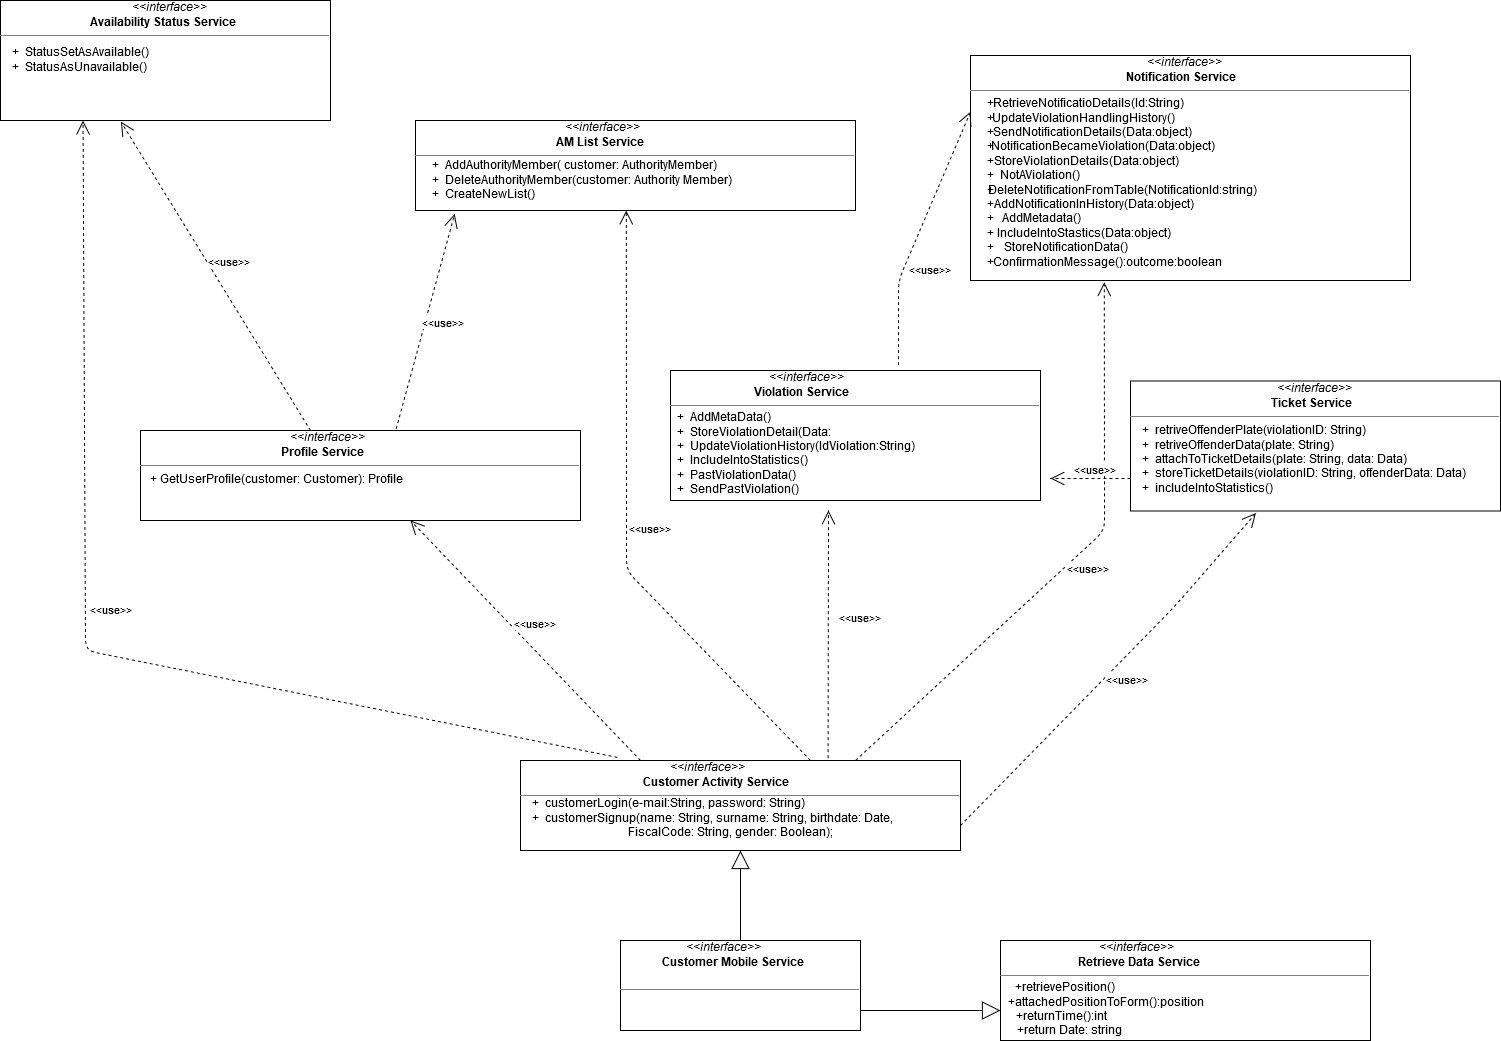
\includegraphics[scale=0.30]{ComponentInterfaces/componentInterface.jpg}


\vspace{2mm}
Figure 2.14: Component Interfaces Customer Mobile Service.
\end{center}
\newpage

\begin{center}
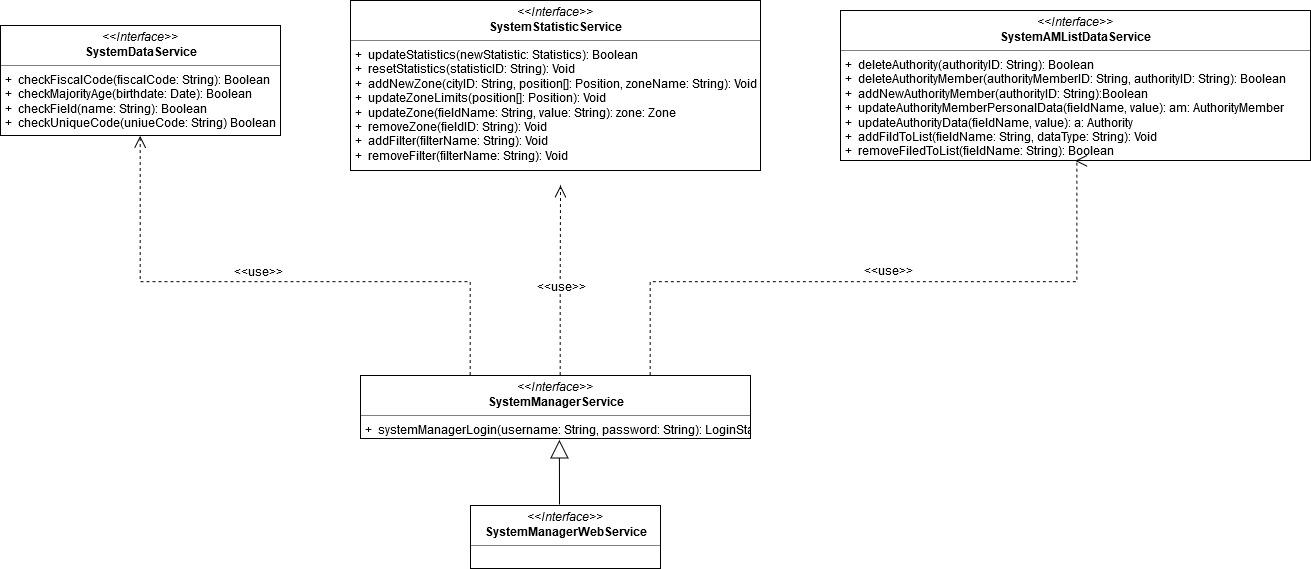
\includegraphics[scale=0.35]{ComponentInterfaces/systemManagerComponentInterface.jpg}


\vspace{2mm}
Figure 2.15: Component Interfaces System Manager Web Service.

\end{center}
\begin{center}
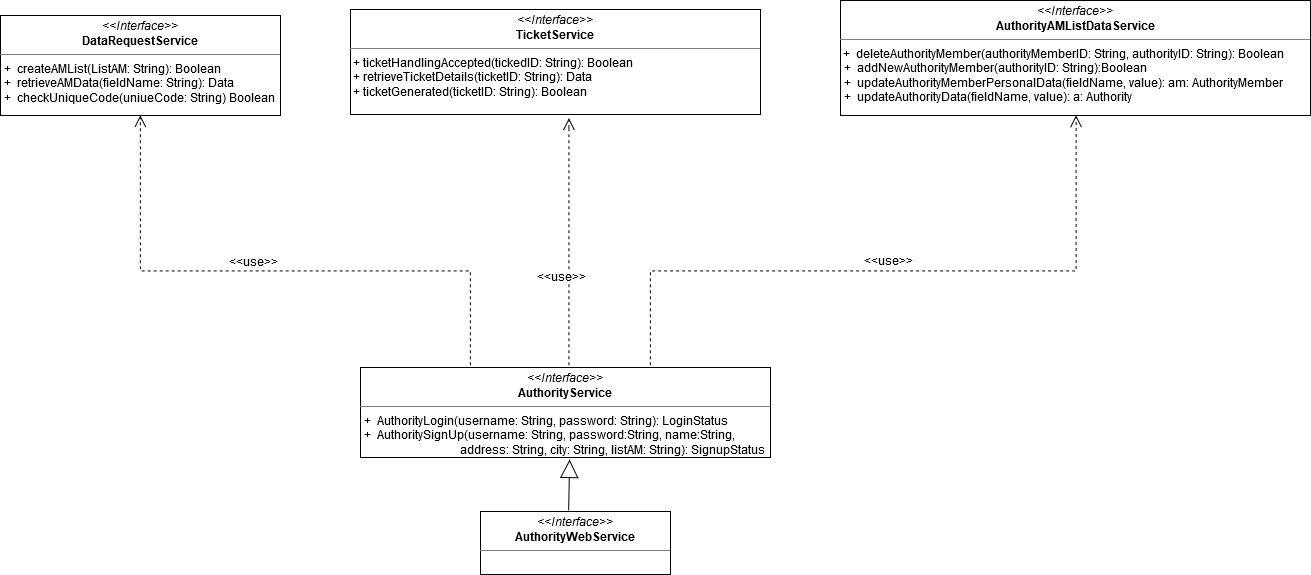
\includegraphics[scale=0.35]{ComponentInterfaces/AuthorityComponentInterface.jpg}


\vspace{2mm}
Figure 2.16: Component Interfaces Authority Web Service.
\end{center}
\newpage

\subsection{Selected architectural styles and patterns}
\vspace{5mm}
\subsubsection{Overall architecture}
For the platform SafeStreets the architectural choice would be a Three Tier Architecture. In the three tier there are the different type of levels. At the highest level there is the presentation tier, which is demanded to show services functionalities and informations for Users, AMs and Authorities, through the mobile application, Authority can access through the dedicated web application too. Just in this tier User, Authority and AM can directly acess, through web and mobile app GUIs.The application tier is enclose by the presentation tier, which acts as an intermediator between the application and the data tiers. The data tier as specified in the RASD is designed to including functionalities of the Hardened Database model, with data persistence and data exposing mechanisms. The data tier also provides to the application tier an interface in order to allow the full management methods on data.
In choosing a three tiers architecture there are pros and cons. The cons are like the high cost to develop this type of architecture, but in the pros there are more important aspects like the best scalability and maintainability aspects.






\newpage
\subsection{Design Patterns}
\vspace{5mm}
\begin{itemize}
\item \textbf{Power and resources consumption constraints}

The application should be optimized to minimize its power consumpation and memory usage during the processes. Then in every design decision should take into account the fact that mobile devices offers limited CPU, memory, storage capacity and battery durability.

\item \textbf{Model View Controller(MVC)}

User interface components are tied with data store components, to agree with MVC design pattern. This pattern is choice since mobile applications' core operation is to retrieve data from a data store and up-date the user interface with the newly requested information based on the user inputs, together with the fact that MVC is one of the most common and effective ways to avoid a dangerous level of coupling between the various parts of the whole system.


\end{itemize}
\newpage
\section{User Interface Design}
\hrule
\vspace{5mm}
\newpage

\newpage
\section{Requirements Tracebility}
\hrule
\vspace{5mm}
While making the design choices presented in this document, the aim is to accomplish all the goals and requirements that have been previously specified in RASD. Below are listed the design components to which requirements and goals are mapped: 






\end{document}
